Cílem této práce bylo zejména optimalizovat sklad tak, aby se maximalizovala propustnost skladu, tedy počet zpracovaných objednávek za jednotku času. To lze chápat také jako zpracování daných objednávek v co nejkratším možném čase. Vyhodnocení je rozděleno na tři části: optimalizaci rozložení produktů, cesty a nakonec jejich kombinaci.

\section{Optimalizace rozložení produktů}
Jak již bylo zmíněno, při optimalizaci tohoto problému se minimalizuje doba potřebná ke zpracování sady objednávek. Na grafu na obrázku~\ref{fig:vyhodnoceniGrafTrain} lze vidět průběh optimalizace pomocí evolučních algoritmů na problému rozřazení $150$ produktů do $200$ slotů, což lze vyjádřit jako kombinatorický problém:
\begin{equation*}
    \label{eq:optVariace}
    V_{150}(200) = \frac{200!}{50!} = 2.593067\text{e}+310.
\end{equation*}
Dále je na grafu vidět také průběh náhodného prohledávání prostoru (\texttt{RAND}) a klasické metodiky (\texttt{Battista a spol.}) použité v práci~\cite{slapSeacomp} -- tato metodika je jednokrokový výpočet mapující nejčastěji kupované produkty do nejvýhodnějších slotů, a proto je konstantní. Nejlépe si vedl genetický algoritmus, kterému se povedlo snížit dobu potřebnou ke zpracování $1000$ objednávek téměř na polovinu ($57\%$). Stejnou optimalizaci avšak v časové doméně (\emph{trade-off} úspěšnosti a času) lze vidět na obrázku~\ref{fig:vyhodnoceniGrafTrainCas}. Vyhodnocení optimalizovaných modelů na testovací sadě vždy cca. odpovídalo úrovni optimalizace na trénovací sadě objednávek. Při kombinatorickém nárůstu možných řešení a při zachování nastavení optimalizátoru a délky optimalizace se kvalita optimalizace snižuje, viz obrázek~\ref{fig:vyhodnoceniPorovnaniOpt} a obrázek~\ref{fig:vyhodnoceniPorovnaniOpt7501000}.

Při analýze průběhů trénování lze vidět, že náhodné prohledávání je z pohledu optimalizace téměř bezvýznamné. Genetický algoritmus velmi rychle konverguje na začátku, ale zhruba od iterace 400 už se vůbec nezlepšuje. Další iterace by tomuto algoritmu tedy už nejspíše nepomohly. Na druhou stranu algoritmus umělých včelstev, optimalizace rojem částic a diferenční evoluce konvergují mnohem pomaleji a při dalších iteracích by se výsledek nejspíše dále lehce zlepšoval. Algoritmus optimalizace rojem částic je z uvedených evolučních algoritmů pro tuto problematiku nejméně vhodný a jako jediný dosahuje horších výsledků, než klasická metoda Battista a spol~\cite{slapSeacomp}. Nejlépe tedy dle očekávání dopadl genetický algoritmus, a sice na všech instancích problému, kterému se podařilo dobu potřebnou pro zpracování objednávek snížit téměř na polovinu.

Vzhledem k tomu, že z porovnání algoritmů pro řešení problematiky SLAP vyšel jako nejlepší genetický algoritmus, pro další experimenty s optimalizací rozložení produktů byl využíván už pouze tento algoritmus. Na snímcích \ref{fig:compCrossover} až \ref{fig:compParams} lze vidět experimenty s různými parametry genetického algoritmu. Z těchto experimentů bylo možné najít nejlepší konfiguraci optimalizátoru, která byla nadále používána a kterou lze vidět v tabulce~\ref{tab:nejConfig}.

\begin{figure*}[t]
    \centering
    \begin{minipage}{0.49\textwidth}
        \centering
        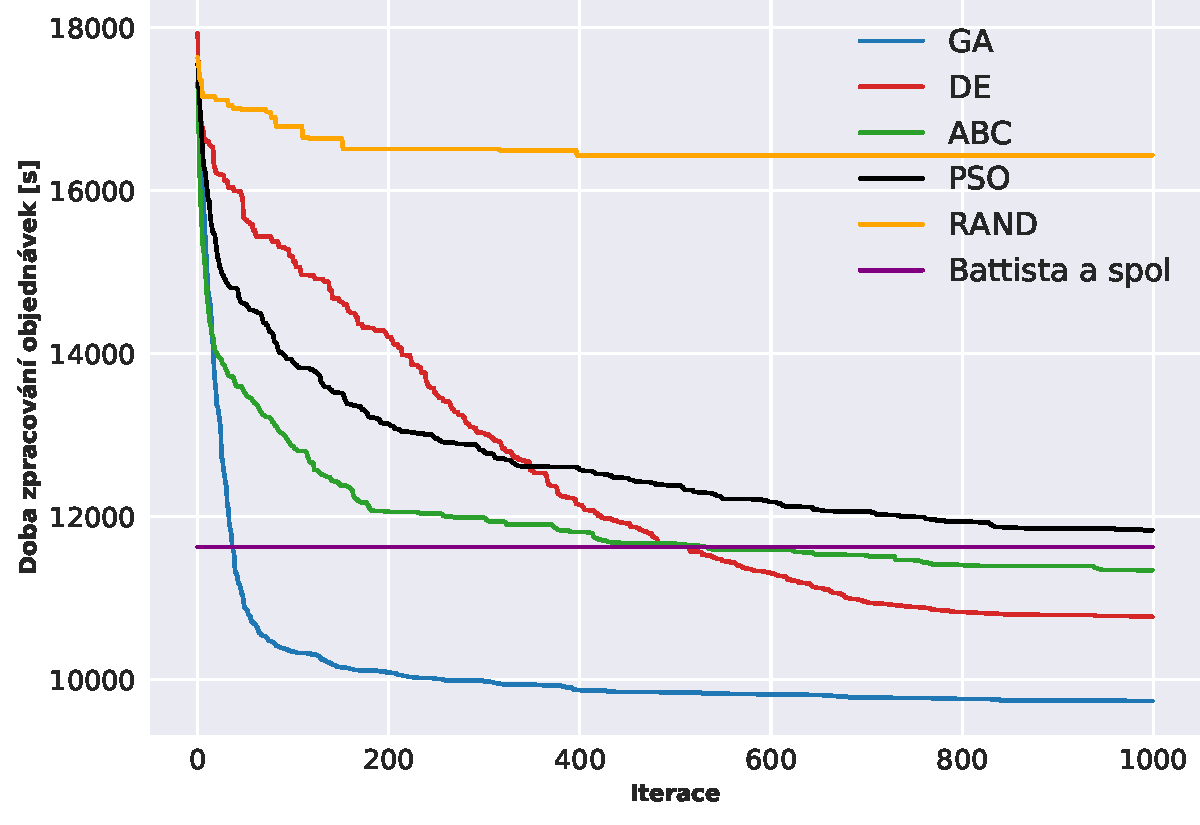
\includegraphics[width=0.99\textwidth]{figures/vyhodnoceni/plotComparisonTrain.pdf}
        \caption{Graf průběhu optimalizace pomocí čtyř evolučních algoritmů, metodiky Battista a spol.~\cite{slapSeacomp} a náhodného prohledávání. Ve všech případech byl použit stejný model skladu (který lze vidět na snímku~\ref{fig:UI_simulator}) a stejné trénovací objednávky. Na vodorovné ose jsou iterace algoritmu a na svislé ose je doba potřebná pro zpracování sady trénovacích objednávek v sekundách. Jedná se o aritmetický průměr \textbf{pěti} běhů na metodu.}
        \label{fig:vyhodnoceniGrafTrain}
    \end{minipage}\hfill
    \begin{minipage}{0.49\textwidth}
        \centering
        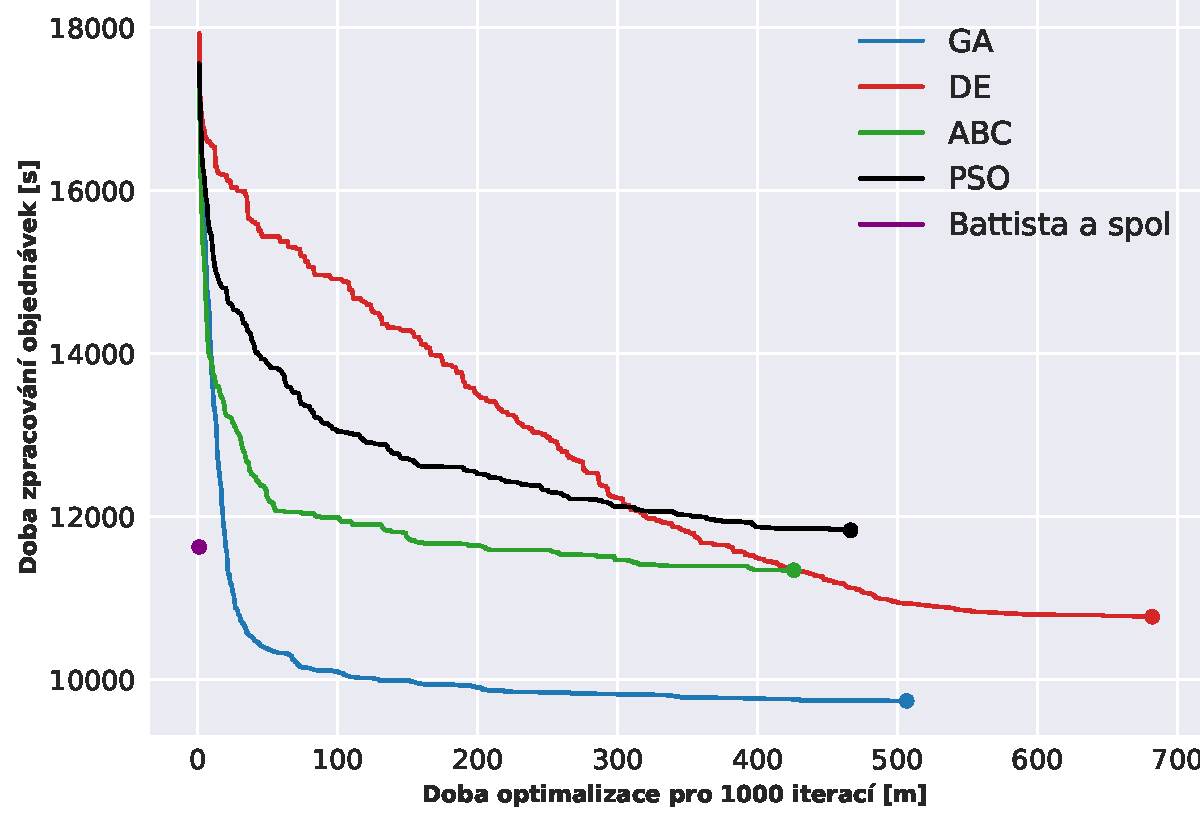
\includegraphics[width=1\linewidth]{figures/vyhodnoceni/plotComparisonTrainTime.pdf}
        \caption{Průběh optimalizace z grafu na obrázku~\ref{fig:vyhodnoceniGrafTrain} v časové doméně, tzn. jak dlouho trvalo 1000 iterací jednotlivých metod. Pokud bychom nebrali v potaz genetické algoritmy, nejvhodnější by byla diferenční evoluce, pokud bychom však měli na optimalizace méně než 400 minut, vhodnější by byl algoritmus umělých včelstev a do 300 minut by vycházel lépe dokonce i algoritmus optimalizace rojem částic.}
        \label{fig:vyhodnoceniGrafTrainCas}
    \end{minipage}\hfill
\end{figure*}

\begin{figure*}[t]
    \centering
    \begin{minipage}{0.49\textwidth}
        \centering
        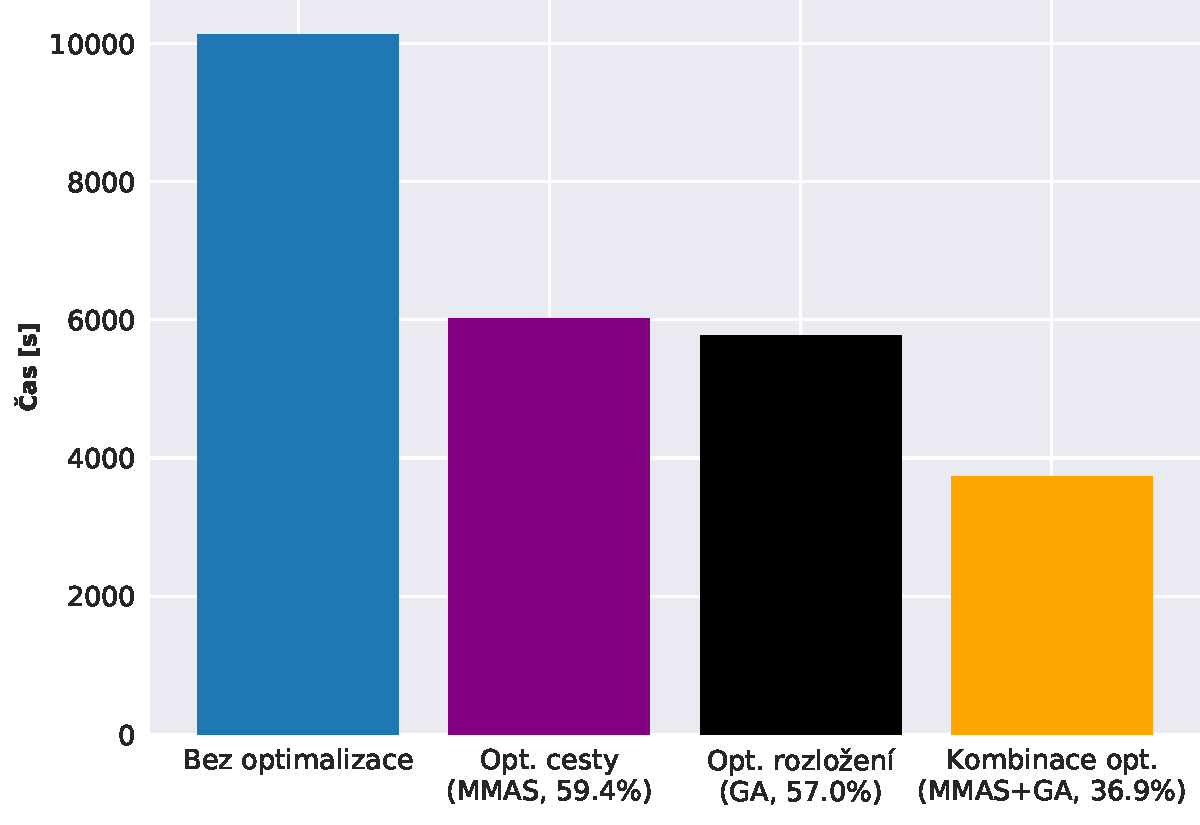
\includegraphics[width=0.99\textwidth]{figures/vyhodnoceni/plotOptimizersComparison.pdf}
        \caption{Sloupcový graf porovnávající optimalizaci cesty pomocí $\mathcal{M}\!\!\mathcal{M}$AS, optimalizaci rozložení produktů pomocí genetického algoritmu a nakonec jejich kombinaci (sklad $200$ produktů, $400$ slotů).}
        \label{fig:vyhodnoceniPorovnaniOpt}
    \end{minipage}\hfill
    \begin{minipage}{0.49\textwidth}
        \centering
        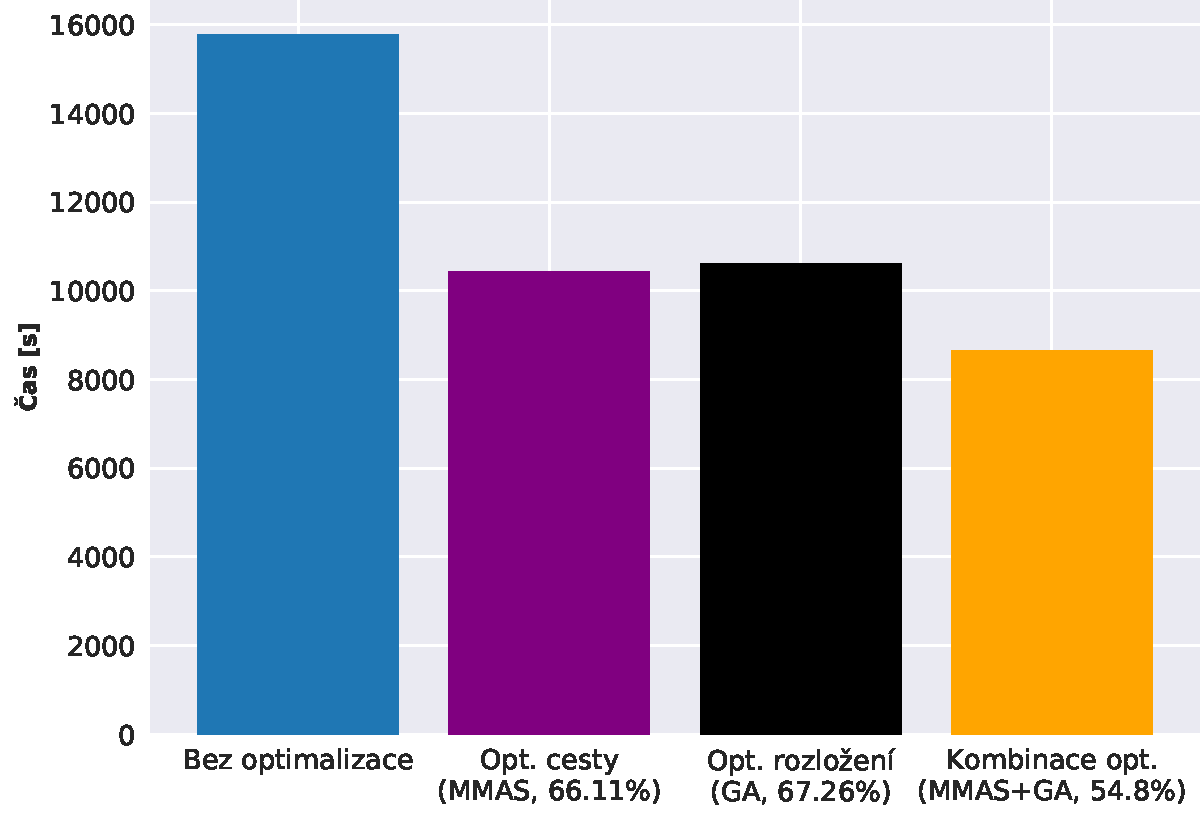
\includegraphics[width=0.99\textwidth]{figures/vyhodnoceni/plotOptimizersComparison7501000.pdf}
        \caption{Sloupcový graf porovnávající optimalizaci cesty pomocí $\mathcal{M}\!\!\mathcal{M}$AS, optimalizaci rozložení produktů pomocí genetického algoritmu a nakonec jejich kombinaci (sklad $750$ produktů, $1000$ slotů).}
        \label{fig:vyhodnoceniPorovnaniOpt7501000}
    \end{minipage}\hfill
\end{figure*}
\begin{figure}[t!]
    \centering
    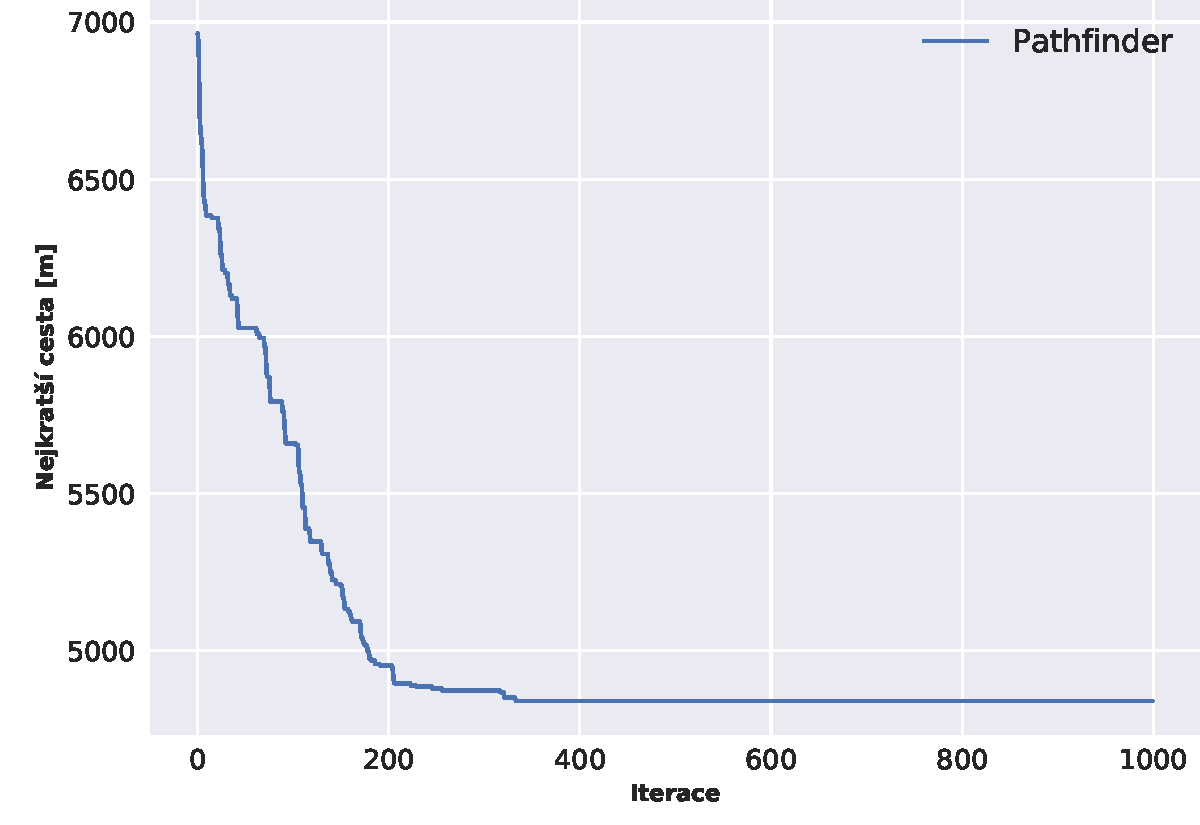
\includegraphics[width=0.7\linewidth]{figures/vyhodnoceni/plotPathFinder.pdf}
    \caption{Graf průběhu hledání optimální cesty pomocí algoritmu $\mathcal{M}\!\!\mathcal{M}$AS na velkém skladu. Jedná se o aritmetický průměr pěti běhů.}
    \label{fig:vyhodnoceniPathFinder}
\end{figure}

\section{Optimalizace cesty}
V rámci této práce byl jako doplněk implementován také nástroj pathfinder, který pomocí mravenčího algoritmu dokáže nalézt optimální cestu objednávky skrze sklad. Na obrázku~\ref{fig:vyhodnoceniPathFinder} lze vidět průběh hledání optimální cesty na skladu o velikosti $200$ lokací, což už je z hlediska skladových politik více než obrovský sklad a tedy nemá význam řešit tento problém pro větší modely skladu. Algoritmus v závislosti na konfiguraci dokáže nalézt optimální řešení (cestu s nejkratší vzdáleností) pro zmíněný sklad do $400$ iterací algoritmu. U skladů typických velikostí je optimální cesta nalezena maximálně do $100$ iterací algoritmu.

\section{Kombinace optimalizací}
Nástroj pathfinder lze použít v rámci simulátoru pro hledání optimálních cest pro objednávky. Vzhledem k tomu, že optimalizátor rozložení používá simulátor pro aproximaci kvality řešení, lze použít všechny tři nástroje zároveň a optimalizovat jednak rozložení produktů a zároveň délku cesty. Na grafu~\ref{fig:vyhodnoceniPorovnaniOpt} lze vidět porovnání (na problému $200$ produktů, $400$ slotů): neoptimalizovaný sklad, nejlepší dosažené výsledky samostatných optimalizací a nakonec kombinace těchto optimalizací. Jak lze vidět, kombinací těchto optimalizátorů lze dosáhnout ještě lepších výsledků, avšak za velice vysokou cenu doby trénování -- optimalizace cesty trvá jednotky minut, optimalizace rozložení jednotky hodin (viz graf na obrázku~\ref{fig:vyhodnoceniGrafTrainCas}) a jejich kombinace pak desítky hodin. Kombinace optimalizací trvající desítky hodin už není v souladu s fungováním moderních skladů, které musí být schopny relativně rychle reagovat na změny požadavků na trhu.
